\chapter{绪论}

\section{课题背景}

依托以互联网为代表的信息技术的高速发展,我国社会当前正处在由传统服务业向现
代服务业全面升级的重要历史进程中。充分利用和结合现代先进的信息技术,提供信息和
知识更加密集、附加值更高的服务是现代服务业的基本要求。互联网作为现代信息服务的
载体,从早期简单的门户网站、搜索引擎,发展到社交网站、即时通信,再到移动搜索、LBS
等移动互联网应用的风靡,在产业规模持续扩大的同时,也不断向各行各业渗透,从早期
的传媒、游戏等行业,到娱乐、零售行业,再到金融、教育和医疗等行业,影响范围还在不
断继续扩大\cite{王晓玲2015我国现代服务业借力}。由此可见,未来服务的基础形态一定是基于互联网的,各行业通过互联网来
提供他们的服务是大势所趋。

跨界服务将跨越不同行业、组织、价值链等边界的服务进行深度融合和模式创新,为用户提供多维度、高质量、富价值的跨界服务,成为现代服务业发
展的重要创新途径。然而,目前针对跨界服务本质规律认知、跨界服务融   
合理论、工程设计方法与运行载体等方面仍然缺少系统研究,缺少充分理
论指导的跨界服务融合实践呈现一定的盲目性,极大影响我国现代服务业
的创新发展。

早期的基于网络的应用服务通常构建于一组相互联系的Web Service 之上。根据W3C
的定义,Web Service 是指用于支持网络内机器之间互操作的软件系统,它通常包含一个机
器可处理的接口描述(一般是WSDL),其它系统按照其接口描述通过SOAP 消息与它进行
交互\cite{verborgh2018web}。Web Service 包含一系列标准化的规范和技术用以支持基于Web 的应用的集成,包
括XML, SOAP, WSDL 和UDDI 等。

Web Service 在早期许多大型企业级软件应用中使用广泛,但由于其相关标准和技术过
于复杂等原因,在如今的新兴互联网应用中已经很少使用了。目前Web API,作为一种更
加灵活和轻量级的解决方案,摒弃了WS 系列的相关复杂标准,得到了广泛的应用\cite{zaveri2017smartapi}。

Web API 如今是Web、物联网、云计算和机器学习应用等的基石\cite{tan2016service}。在Web 应用领域,
随着前后端分离架构的普及,很多Web 应用的界面背后都是由相关的Web API 在直接支
持动态的数据获取和功能访问。在物联网应用中,智能设备和终端也经常会用到诸如广告、
社交网络、消息和支付等Web API\cite{gorla2014checking,viennot2014measurement}。在云计算领域,云服务提供商提供的诸如计算、存
储、消息和数据库等基础服务,都是以Web API 形式供使用者按需调用。在机器学习应用
中,也有许多诸如谷歌翻译这样的Web API,使得开发者无需收集数据、训练模型,也能
直接使用顶尖的图像分类、语音识别和机器翻译等能力。

正是意识到Web API 具有的无限潜能,许多公司选择成立自己的开放平台,开放自家
的部分Web API,一起共建更大的服务生态,实现开放共享、互利共赢。作为最大的Web
API 收录网站,ProgramWeb 网站已经收录了12453 个Web API 和4593 个组合服务。当然
还有许多收费的、企业内部使用的Web API 远远没有收录。Web API 背后所代表的数据和资源,已经促成了所谓API 经济的形成。出现了以京东万象、聚合数据等为代表的各种API
商店。许多供应商仅仅靠提供Web API 就能获得可观的收入,比如SalesForce, AWS。[7]
尽管Web API 目前已经得到了非常广泛的应用,然而在使用Web API 的过程中仍然存
在很多问题。

\begin{figure}[htbp]
  \centering
  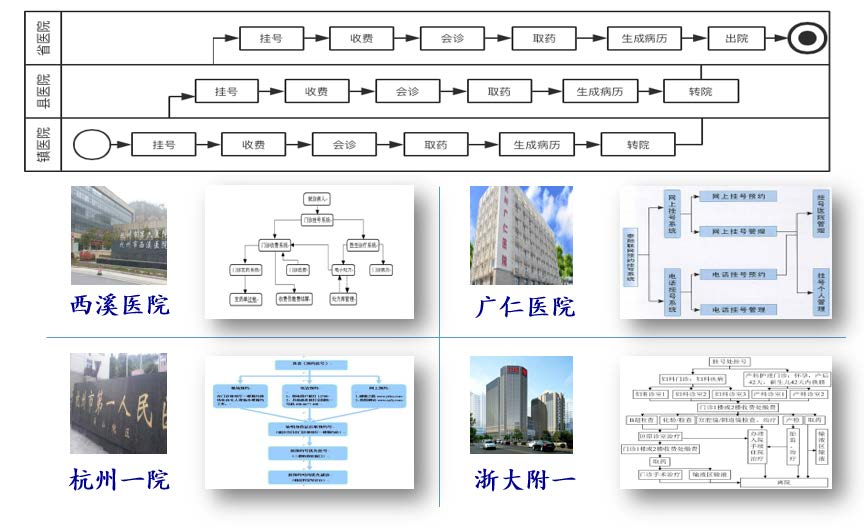
\includegraphics[scale=1]{./images/hospitalRunningModel.jpg}
  \caption{传统医院经营模式下,各家医院标准不一}
  \label{fig:hospitalRunningModel}
\end{figure}

首先,Web API 的描述问题:许多Web API 缺乏有效的描述文档,这给其使用者带来
了很大的障碍。另外,Web API 缺乏统一的描述规范,导致各个公司、组织等都在使用自定
义的、不一致的描述方式,这对于各企业、组织间Web API 的集成和交互式非常不利的,如图\ref{fig:hospitalRunningModel}所展示的,各个地方的医院系统标准不一。再
有就是现在的Web API 描述文档,都是针对人类用户的,缺乏机器可理解性,这对于Web
API 的高效应用,诸如自动组合等方面都是很不利的。

其次,Web API 当前的使用体验问题:用户需要仔细阅读相应的说明文档,然后往往
还需要根据所提供的Web API 的请求和响应等,结合自己的实际需要,进行一层定制或者
包装工作,要正确的使用一个Web API 来获得满足自己需求的结果其实并不容易。

然后,Web API 的选择问题:在很多功能类似的服务中选择一个合适的对很多用户来
说是个挑战。

最后,Web API 的演化问题:服务提供者经常需要升级他们的服务,尽管他们力求做
到向后兼容,但往往还是会或多或少的破坏原来的Web API 接口,服务使用者不得不被迫
修改他们的应用代码以适应新的Web API 的要求,这经常是一项枯燥又繁琐的工作。

本文从服务使用者的角度出发,为解决上述Web API 使用过程中的问题,提出了服务
映射的方法,并开发了相应的系统来支持用户更好的使用服务。

\section{研究意义}
现代服务业是中国经济发展战略中的重要组成部分,也是衡量一个国家经济发展水平
的重要标志。推动现代服务业的发展壮大已成为当前中国经济发展的重要目标和关键动力。
服务计算作为现代服务业发展的重要技术基础,需要结合现代服务业发展的具体场景和具
体问题进行深入的研究和应用。本文依托于国家重点研发计划专项《现代服务业共性关键
技术研发及应用示范》的子课题《跨界服务集成方法与支撑载体》,围绕在研究跨界服务集
成和交互过程中发现的Web API 描述文档缺乏、描述方式不一致等导致的集成困难、难以
交互,以及服务使用者使用Web API 过程中遇到的门槛较高、难以上手,需要根据自身需
求进行包装和定制操作,同类服务难以选择,以及Web API 演化导致的应用失败等实际问
题进行了深入的研究和分析,提出了一套以服务映射、流程映射为基础的解决方案,并
开发了对应的原型系统,不但能够有效解决跨系统的Web API 集成问题,而且提出了以用户为中心的Web API 的使用方式,能够大大简化和改善用户使用Web API 的流程和体验,
还能够避免Web API 演化带来的应用失败的问题,因此本文的研究具有重要的意义。如图\ref{fig:yilianti}
所示,医联体环境下医院经营模式,集成了海量的服务,对用户暴露统一的接口,大大简化了用户的操作。

同时,近年来,数字经济已成为全球经济的重要驱动力,“工业+技术”的无限融合不断为市场经济注入新的动力。
在这一发展的浪潮中,企业将大多数业务以Web服务的形式部署在网络中,并为实现复杂业务提供了最基本的功能单元。
 最初,这种复杂的业务模型通常是在企业内部实现的,即不同部门根据预定的任务划分提供自己的服务,最终实现复杂而完整的产品。 
 但是,随着开发人员要求日益复杂和全球分工明确,单个企业可以提供的服务将不再能满足市场需求。 因此,需要跨企业边界的服务流程来实现业务增值。

 在当前情况下,当开发人员想要实施复杂的业务时,他需要分析如何首先将业务划分为几个模块,
 以及每个模块需要什么服务。之后,他需要构建服务流程并基于QoS进行服务选择。
 上述两个步骤中的每一个都消耗大量的劳动力,并且需要非常丰富的领域专家知识,这将带来巨大的代价。
 此外,当选择的服务变得不稳定,整个服务流程链将进入又一个不稳定的状态,
 这暴露了整个业务在很长一段时间内不稳定的风险。想象一下医院要发布一站式在线挂号服务的情况,
 显然,医疗卫生专业人员对Web服务的工作原理知之甚少,因此他们将这个业务项目委托给服务解决方案提供商。
 服务解决方案提供商首先花费大量时间来确定医院的特定业务需求,然后,他们使用“部门信息获取”,“专家信息获取”,
 “注册资源获取”,“注册”和“账单支付”五个功能模块对整个业务的服务流程进行建模。
 在此基础上,他们在服务注册中心检索了服务。在评估了服务的QoS之后,
 他们最终选择了例如分别由服务提供商A,B,C,D,E提供的服务a,b,c,d,e以完成挂号业务。但是,注册服务上线几个月后,服务提供商B突然出于某种原因宣布关闭其服务b。
 因此,医院只能再次找到先前的服务解决方案提供商,并重做服务选择和业务流程的构建。在此期间,由于挂号业务的中断,给医院造成了巨大损失。

\begin{figure}[htbp]
  \centering
  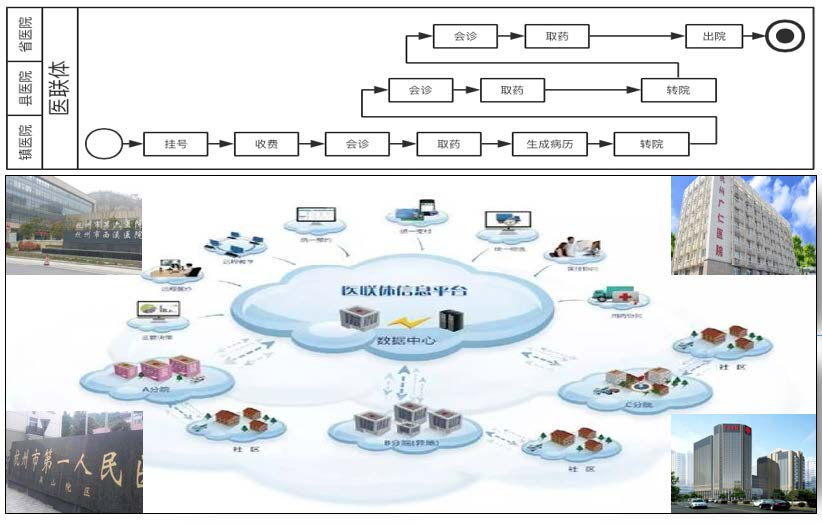
\includegraphics[scale=1]{./images/yilianti.jpg}
  \caption{医联体环境下医院经营模式图}
  \label{fig:yilianti}
\end{figure}

\section{国内外研究现状}

